\section{Diferencia entre el MaxEnt y el AssMap}
No tenemos ninguna razón para asegurar que el estado de máxima entropía y el estado asignado por promedio son el mismo. Por el momento, podemos compararlos numéricamente. Sea $\rho$ un estado alineado en $z=0.5$. 
\begin{figure}[h!]
    \centering
    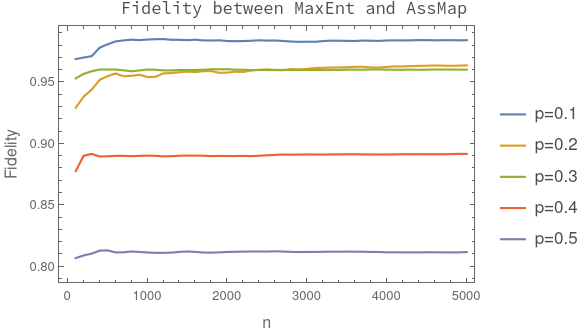
\includegraphics[width=0.6\linewidth]{general/figures/fidelityMaxEntAssMap_vs_n.png}
    \caption{Fidelidad entre el estado de máxima entropía y el estado asignado por promedio como función del número de estados usados en el promedio, para diferentes valores del parámetro $p$.}
    \label{fig:FidMaxEntAssMapN}
\end{figure}
La figura \ref{fig:FidMaxEntAssMapN} muestra que la fidelidad entre ambos estados parece constante siempre que $n>1000$, y que la verdadera dependencia se halla sobre el parámetro $p$. Veamos, pues, la fidelidad entre ambos estados como función de $p$, con $n=1000$.
\begin{figure}[h!]
    \centering
    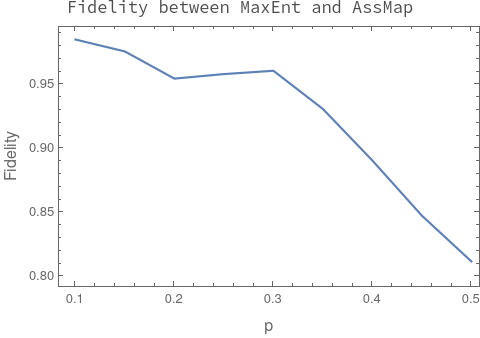
\includegraphics[width=0.6\linewidth]{general/figures/fidelityMaxEntAssMap_vs_p.png}
    \caption{Fidelidad entre el estado de máxima entropía y el estado asignado por promedio como función de $p$.}
    \label{fig:FidMaxEntAssMapP}
\end{figure}
La figura \ref{fig:FidMaxEntAssMapP} es algo burda, y puede que requiera más puntos y observaciones, pero parece revelar que los estados tienden a ser el mismo cuando $p\rightarrow 0,1$. Asumo aquí simetría respecto a $p=0.5$. \notaAd{Bastará con generar puntos entre 0.5 y 1}.